\glsresetall

\chapter{Referencial Teórico}
\label{chap.background}

Neste capítulo serão apresentados conceitos fundamentais para o entendimento do trabalho. A \autoref{sec.lw} apresenta uma visão geral da evolução dos processadores, partindo dos \singlecores até os \lws. A \autoref{sec.nanvixos} apresenta o \nanvix, \so distribuído que será utilizado no desenvolvimento deste trabalho. A \autoref{sec.virtualizacao} descreve detalhes importantes sobre a virtualização e migração de processos.

\section{Dos \singlecores aos \Lws}
\label{sec.lw}

O aumento de desempenho dos sistemas computacionais manteve-se como uma necessidade constante para o avanço da ciência em vários setores: astrologia, biologia, engenharia, etc. Até tempos atrás, esse objetivo era alcançado através do aumento da frequência de relógios do núcleo de processamento, do avanço na tecnologia dos semicondutores e do acréscimo do número de transistores em um \chip~\cite{amrouch2018negative}. Atualmente, nós já chegamos ao limite físico que impede a aplicação de parte dessas técnicas. Além da dificuldade de garantir a dissipação de calor à medida que a frequência aumenta, o número de transistores que conseguimos colocar em uma mesma área de um \chip chegou a um limite físico, \ie o tamanho dos transitores alcançou a escala atômica.

Como alternativa para a continuidade nos avanços de poder computacional, foram exploradas novas técnicas~\cite{fuller2011computing,gepner2006multi}. Em especial, foram desenvolvidas arquiteturas paralelas, que exploram o poder de processamento paralelo, o qual é atingido pela execução de múltiplos \cores simultaneamente~\cite{gepner2006multi}. Essas novas arquiteturas são classificadas de acordo com a maneira com que conseguem manipular os dados. São elas:
\begin{inlinelist}
    \item \sisd;
    \item \simd;
    \item \misd;
    \item \mimd.
\end{inlinelist}
Neste trabalho, estamos interessados nas arquiteturas que suportam cargas de trabalho \mimd. 

Algumas dessas arquiteturas são ilustradas pela \autoref{fig.mimd}. A \autoref{fig.mimd1} apresenta uma visão conceitual de um multiprocessador de memória compartilhada, em que os múltiplos \cores têm acesso a toda a memória, a qual é compartilhada por todos os núcleos. A \autoref{fig.mimd2} exemplifica um multicomputador com troca de mensagens, em que conjuntos compostos por \cores e memória são interconectados por uma rede em \chip. As memórias são acessíveis somente pelos \cores pertencentes ao seu conjunto e os \cores se comunicam entre si via troca de mensagens através da rede que interconecta todos os conjuntos. Já a \autoref{fig.mimd3} evidencia um sistema distribuído de grande escala, em que computadores são conectados através de uma \wan com o intuito de formar um sistema distribuído.
% \todo{Sobre a fig mimd, não precisa ser agora mas: mudar o texto nas imagens para pt-br}

Neste contexto, a classe de processadores \lws destacam-se por atrelar alto poder de processamento com eficiência energética~\cite{francesquini2015}. Os \lws são classificados como \mpsoc e suas arquiteturas apresentam as seguintes características:
\begin{enumerate}[label=(\roman*)]
    \item Integrar de centenas à milhares de núcleos de processamento operando a baixas frequências em um único \chip;
    \item Processar cargas de trabalho \mimd;
    \item Organizar os núcleos em conjuntos, denominados \clusters, para compartilhamento de recursos locais;
    \item Utilizar \nocs para transferência de dados entre núcleos ou \clusters;
    \item Possuir sistemas memória distribuída restritivos, compostos por pequenas memórias locais; e
    \item Apresentar componentes heterogêneos (\cclusters e \ioclusters).
\end{enumerate}

\begin{figure}[t]
	\centering
	
    \caption{Exemplos de arquiteturas \mimd.}%
	\subcaptionminipage[fig.mimd1]%
                   {.25\textwidth}
                   {multiprocessador de memória compartilhada.}
                   {\includesvg[width=\textwidth]{content/images/mimd-1.svg}}
	\qquad
	\subcaptionminipage[fig.mimd2]
                   {.25\textwidth}
                   {multicompudator com troca de mensagens.}
                   {\includesvg[width=\textwidth]{content/images/mimd-2.svg}}
    \qquad
    \subcaptionminipage[fig.mimd3]
                   {.25\textwidth}
                   {sistema distribuído de grande escala.}
                   {\includesvg[width=\textwidth]{content/images/mimd-3.svg}}

    \fonte{Adaptado de \citeonline{tanenbaum:4ed}}
    \label{fig.mimd}
\end{figure}

Alguns exemplos comerciais bem sucedidos de \lws são o \mppa~\cite{dinechin:2013}, PULP~\cite{pulp} e \taihulight~\cite{fu2016sunway}.
%
Especificamente, nós utilizamos o processador \mppa para o desenvolvimento deste trabalho. A \autoref{fig.arch-mppa} apresenta uma visão geral do processador \mppa e suas peculiaridades, tais como:

\begin{enumerate}[label=(\roman*)]
    \item Integrar 288 núcleos de baixa frequência em um único \textit{chip};
    \item Possuir núcleos organizados em 20 \clusters;
    \item Dispor de 2 \nocs para transferência de dados entre \clusters, uma para controle e outra para dados;
    \item Possuir um sistema de memória distribuída composto por pequenas memórias locais, \eg \sram de 2 MB;
    \item Não dispor de coerência de \cache em \hardware;
    \item Apresentar heterogeneidade, como \clusters destinados à computação (\cclusters) e \clusters destinados à comunicação com periféricos (\ioclusters).
\end{enumerate}

\begin{figure}[t]
    \centering
    \caption{Visão arquitetural do processador \mppa.}
    \includegraphics[width=0.6\linewidth]{content/images/arch-mppa-gs.png}
    \fonte{\citeonline{penna:sbesc19}}
    \label{fig.arch-mppa}
\end{figure}

\section{\nanvixos}
\label{sec.nanvixos}

O \nanvix\footnote{Disponível em https://github.com/nanvix} é um \os distribuído e de propósito geral que busca equilibrar desempenho, portabilidade e programabilidade para \lws~\cite{penna:sbesc19}. O \kernel do \nanvix é estruturado em três camadas de abstração. São elas:
\begin{description}
    \item [\nanvix \hal]
         é a camada mais baixa que abstrai e provê o gerenciamento dos recursos de \hardware sobre uma visão comum~\cite{penna:hal}. Entre esses recursos estão: \cores, \tlbs, \cache, \mmu, \noc, interrupções, memória virtual e recursos de \io. De maneira geral, esta camada provê abstrações ao nivel do \core, \cluster e comunicação/sincronização entre \clusters~\cite{penna:thesis}. A Figura \ref{fig.hal-overview} ilustra a estrutura interna da \hal do \nanvix.
    \item [\nanvix \Microkernel]
        é a camada intermediária que provê gerenciamento de recursos e os serviços mínimos de um \os em um \cluster. Entre esses serviços se encontram o gerenciamento de \threads e memória, controle de acesso à memória, interface para chamadas de sistema e a comunição entre processos. As chamadas de sistema podem ser executadas localmente, caso acessem dados \rdo ou alterem estruturas internas do \core, ou remotamente pelo \mcore, que atende à requisição e libera o \score requisitante ao término da chamada~\cite{penna:thesis}. Essa característica adjetiva o \microkernel como assimétrico. A Figura \ref{fig.microkernel-overview} ilustra a estrutura interna do \microkernel do \nanvix.
    \item [\nanvix \Multikernel]
        é a camada superior que provê os serviços mais complexos de um \os e dispõe uma visão a nível do processador em si. Os serviços são hospedados em \ioclusters, \ie isolados das aplicações de usuário. Os serviços atendem as requisições vindas dos processos de usuário através de um modelo cliente-servidor. As requisições e respostas são enviadas/recebidas através de passagem de mensagem via \noc. Os serviços dessa camada podem ser entendidos como fontes de informação que mantém a execução dos processos consistentes no processador, tendo em vista a natureza distribuída da memória nessas arquiteturas. Alguns serviços incluídos no \nanvix são mecanismos de \spawn de processos e gerenciamento de nomes lógicos dos processos à fim de abstrair a localização dos processos no processador. A Figura \ref{fig.multikernel-overview} ilustra o \multikernel do \nanvix.
\end{description}

\begin{figure}[bt]
    \centering
    \caption{Estrutura interna da \hal do \nanvix.}
    \includesvg[width=0.9\linewidth]{content/images/hal.svg}
    \fonte{\citeonline{penna:thesis}}
    \label{fig.hal-overview}
\end{figure}

\begin{figure}[bt]
    \centering
    \caption{Estrutura interna do \microkernel do \nanvix.}
    \includesvg[width=0.9\linewidth]{content/images/microkernel.svg}
    \fonte{\citeonline{penna:thesis}}
    \label{fig.microkernel-overview}
\end{figure}

\begin{figure}[bt]
    \centering
    \caption{Estrutura interna do \multikernel do \nanvix.}
    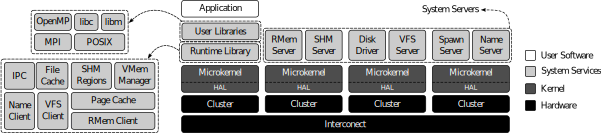
\includegraphics[width=0.9\linewidth]{content/images/multikernel.png}
    \fonte{\citeonline{penna:thesis}}
    \label{fig.multikernel-overview}
\end{figure}


Em sua abordagem original, os processos no \nanvix são estáticos, \ie cada \cluster possui apenas um processo. Desse modo, uma vez que o processo inicia sua execução em um \cluster, este finalizará a execução no mesmo \cluster. 
Isso torna o processo dependente do \cluster que o executa, fazendo com que a comunicação entre processos esteja atrelada aos \clusters nos quais os processos são executados (e não aos processos em si). A falta de mobilidade dos processos nesse modelo pode trazer sobrecargas ao processador, afetando diretamente o desempenho do sistema quando múltiplas aplicações estão em execução simultânea no processador. No caso de aplicações paralelas, compostas por múltiplos processos (ou \textit{threads}) que se comunicam, a disposição dos processos (ou \textit{threads}) nos \clusters se torna importante, pois a comunicação entre \clusters próximos é mais rápida e resulta em menor consumo energético do processador. Sendo assim, melhorar a mobilidade e a disposição dos processos no processador possibilitaria melhorar o gerenciamento dos recursos do mesmo. 

Um exemplo de mobilidade é viabilizar a migração de processos entre \clusters. Neste contexto, este trabalho explora essa desassociação entre o processo e o \cluster que o executa. Deste modo, nós aumentamos a mobilidade dos processos, permitindo a migração de processos entre os \clusters do processador.

\subsection{Abstrações de Comunicação do \nanvix}

O \nanvix dispõe de três abstrações de comunicações para transferência de dados e sincronização entre \clusters~\cite{penna:thesis}. Nas próximas seções serão detalhadas as três abstrações principais do \nanvix.

% \begin{figure}[tb]
% 	\centering
%     \caption{Fluxo de execução da abstração \sync.\label{fig.sync}}
% 	\subcaptionminipage[fig.sync1n]%
%                    {.44\textwidth}
%                    {Modo $1:N$.}
%                    {\includesvg[width=\textwidth]{content/images/sync-1-n.svg}}
% 	\qquad
% 	\subcaptionminipage[fig.syncn1]
%                    {.44\textwidth}
%                    {Modo $N:1$.}
%                    {\includesvg[width=\textwidth]{content/images/sync-n-1.svg}}
%     \fonte{\citeonline{penna:thesis}}
% \end{figure}

\begin{description} 

    \item[\sync.] A abstração \sync suporta a sincronização entre \textit{kernels}. Através dela um processo pode esperar um sinal, que pode ser disparado por outro processo remotamente através das interfaces \noc. Essa abstração é muito utilizada na inicialização do sistema para garantir um estado inicial consistente dos subsistemas do \os~\cite{penna:thesis}.

% O \sync pode ser operado duas maneiras distintas: o modo $1:N$ e $N:1$. No modo $1:N$ (\autoref{fig.sync1n}) um nó envia uma notificação a múltiplos nós, que estão esperando pelo sinal e são liberados após o recebimento do sinal. Em contraste, no modo $N:1$ (\autoref{fig.syncn1}), múltiplos nós enviam uma notificação a um único nó, que é liberado após o recebimento do sinal de todos os outros nós envolvidos~\cite{penna:thesis}.

% \begin{figure}[t]
%     \centering
%     \caption{Fluxo de execução da abstração \mailbox.}
%     \includesvg[width=0.5\linewidth]{content/images/mailbox.svg}
%     \fonte{\citeonline{penna:thesis}}
%     \label{fig.mailbox}
% \end{figure}

    \item[\mailbox.] A abstração \mailbox é responsável pelo suporte ao envio de mensagens de controle através da troca de pequenas mensagens de tamanho fixo. A abstração segue a semântica $N:1$ e funciona da seguinte forma: um nó (destinatário da mensagem) possuí uma \mailbox, da qual lê mensagens, e múltiplos nós (remetentes da mensagem) podem escrever nessa \mailbox~\cite{penna:thesis}.

% \begin{figure}[t]
%     \centering
%     \caption{Fluxo de execução da abstração \portal.}\label{fig.portal}
%     \includesvg[width=0.5\linewidth]{content/images/portal.svg}
%     \fonte{\citeonline{penna:thesis}}
% \end{figure}

\item[\portal.] A abstração portal suporta a troca de mensagens grandes e segue a semântica $1:1$. A abstração pode ter uso em diversos cenários que exigem grandes transferências de dados entre \clusters~\cite{penna:thesis}.
\end{description}

\section{Virtualização}
\label{sec.virtualizacao}
A virtualização pode ser entendida como uma técnica de abstração de \hardware que permite a criação de uma versão virtual de um ambiente, como computadores, \sos, sistemas de armazenamento, redes, aplicações, etc. Nesse cenário, muitas vezes é possível a criação de múltiplas instâncias dessa versão virtual, as quais competem pelos recursos físicos/reais. A virtual ização pode ser classificada em três grupos principais: a virtualização total; a para-virtualização e a virtualização a nível de processo. Além disso, o isolamento e independência das instâncias virtuais garantem à virtualização algumas vantagens muito exploradas atualmente, especialmente em ambientes \cloud~\cite{manohar2013survey}. Dentre elas: flexibilidade, portabilidade, escalabilidade e segurança.

O conceito de virtualização pode ser traçado desde a década de 50, durante a época dos \mainframes e do emergente conceito de memória virtual~\cite{campbell2006introduction}. Nesse período, a preocupação era tornar um recurso físico acessível a múltiplos usuários simultaneamente. Essa motivação sustentou a evolução da virtualização, levando ao surgimento das \vms e dos \hypervisors. Com o tempo, viu-se o surgimento de novos projetos, como o M44/44x da \ibm, responsável pelo nascimento de um novo \design para os sistemas de tempo compartilhado. Nessa nova estrutura, a máquina central repartia seus recursos em diversas instâncias de \vms, que eram utilizadas por múltiplos usuários simultaneamente.

O retorno das pesquisas sobre virtualização ocorreu mais recentemente, na década de 90~\cite{campbell2006introduction}. Essa foi a época em que o número de serviços e servidores cresceu bruscamente. Naturalmente, com o aumento do número de servidores e aplicações hospedadas nesses servidores, a necessidade de gerenciamento desses recursos também aumentou. Nesse cenário, a virtualização mostrou-se uma solução viável por permitir que diversas \vms compartilhassem um único servidor mantendo, ainda assim, a independência dos serviços providos por essas \vms encapsulados. Isso significa que a interrupção ou quebra de um serviço não afeta os demais graças à virtualização, que garante uma maior flexibilidade e escalabilidade. Por consequência, a virtualização reduziu os custos de manutenção e operação, já que os recursos de \hardware foram utilizados de maneira mais eficiente e houve a redução na quantidade de máquinas físicas para gerenciar.

Atualmente, a tendência de uso de \vms em servidores continua crescente. Hoje, a virtualização de servidor é uma das formas mais comuns de virtualização, sendo utilizada em ambientes \cloud para garantir o suporte à execução de múltiplas aplicações, possivelmente em \oss distintos sobre o mesmo \hardware~\cite{manohar2013survey}.

\subsection{Virtualização total}
A virtualização total tem como objetivo abstrair o \hardware de um computador como um todo. Cada instância executa isoladamente e independentemente uma das outras. Neste tipo de virtualização, é utilizado um \vmm, também conhecido como \hypervisor, o qual, na virtualização total, é classificado como tipo 1~\cite{campbell2006introduction}. O \hypervisor tipo 1 é um \software que roda no nível mais privilegiado e atua como um intermediário entre o \hardware e os múltiplos \sos. O \hypervisor tipo 1 é o único programa do sistema que possui o acesso ao \hardware físico, \eg \cpu, memória e armazenamento, sendo responsável por gerenciar esses recursos de \hardware para cada instância virtual da máquina virtualizada~\cite{sweeney2016virtualization}.

\subsection{Para-virtualização}
De forma similar à virtualização total, o objetivo da para-virtualização também é a abstração da máquina em sua totalidade. Contudo, em contraste com a virtualização total, na para-virtualização uma única instância da máquina executa um \so, chamado de \so hospedeiro, que detém o acesso ao \hardware. Enquanto as demais instâncias executam seus respectivos \sos, chamados de \sos convidados, sob o intermédio de um \hypervisor (\vmm) tipo 2, que pode ser entendido como um processo regular do \so hospedeiro~\cite{campbell2006introduction}. Sendo assim, o \hypervisor tipo 2 atua como um intermediário entre o \so convidado e o \so hospedeiro. O \so hospedeiro reconhece as requisições do \so convidado e gerencia os recursos de \hardware deste~\cite{sweeney2016virtualization}.

\subsection{Virtualização a Nível de Processo e Conteinerização}
Virtualizar um processo ou aplicação é o processo de desacoplar a execução de um processo do sistema que o executa. Nesse contexto, o processo tem uma visão virtual única do sistema, de modo que a execução de cada aplicação ocorre independentemente uma da outra.

Neste tipo de virtualização, cada aplicação é isolada em um ambiente virtual, também conhecido como contêiner, no qual estão contidas todas as bibliotecas, arquivos e configurações necessárias para a execução da aplicação. Como não é necessária a criação de um \so para cada aplicação, a virtualização se torna muito mais leve, \ie tem um impacto menor na memória.

O fato do modelo de conteinerização exigir muito menos espaço e complexidade arquitetônica para existir torna este modelo muito atrativo para sistemas com restrições de memória, tal qual os \lws.

\subsection{Outros Tipos de Virtualização}
% \begin{enumerate}[label=(\roman*)]
%     \item Virtualização de \desktop: usuários acessam o ambiente computacional, ou \desktop, remotamente. O poder e recursos computacionais estão centralizados, mas os pontos de acesso podem ser diversos. Também é conhecido como \vdi.
%     \item Virtualização de armazenamento: múltiplos dispositivos de armazenamento são unificados sob uma mesma visão de dados \ie os dados estão dispersos, mas aparecem como um único conjunto de dados compartilhados.
%     \item Virtualização de rede: múltiplas redes virtuais, cada uma com seu conjunto de recursos (como roteadores, \switches e \firewalls) operam sobre uma mesma rede física. Isso permite melhor gerenciamento de tráfego e otimizção.
% \end{enumerate}
\begin{description}
    \item [Virtualização de \desktop:] usuários acessam o ambiente computacional, ou \desktop, remotamente. O poder e recursos computacionais estão centralizados, mas os pontos de acesso podem ser diversos. Também é conhecido como \vdi.
    \item [Virtualização de armazenamento:] múltiplos dispositivos de armazenamento são unificados sob uma mesma visão de dados \ie os dados estão dispersos, mas aparecem como um único conjunto de dados compartilhados.
    \item [Virtualização de rede:] múltiplas redes virtuais, cada uma com seu conjunto de recursos (como roteadores, \switches e \firewalls) operam sobre uma mesma rede física. Isso permite melhor gerenciamento de tráfego e otimizção.
\end{description}

\subsection{Virtualização no \nanvix}
% \mytodo{problemas dos lws, pq a virtualização é dificultada?, ideia geral do microkernel e outros sistemas que vao ser virtuzalizados}

O foco deste trabalho é desacoplar a execução de um processo do \cluster em que ele é alocado, tornando possível a execução do processo em qualquer \cluster. Para isso, é necessário que seja introduzido o conceito de virtualização no \nanvix.

É importante destacar que o \nanvix é um \so para \lws, os quais apresentam um sistema de memória restritivo, com memória local pequena. Isso torna difícil a virtualização, pois a criação de uma duplicata inteira do \so para cada processo é inviável. Sendo assim, a utilização de contêineres se torna atrativa. 

Na abordagem original do \nanvix, o processo é dependente do \cluster em que é alocado, o que afeta o suporte a migração e diminui a eficiência computacional, como detalhado na \autoref{sec.nanvixos}. Nesse contexto, a virtualização torna-se útil por aumentar a mobilidade dos processos, o que possibilitaria o gerenciamento da distribuição dos processos no processador. Especificamente, este trabalho explora um modelo mais leve de virtualização para \lws baseada em contêineres. Contêineres são executados pelo \os como aplicações virtuais e não incluem um \os convidado, não sendo necessária a criação de duplicatas de \sos e resultando em um menor impacto no sistema de memória e requisitando menor complexidade do \hardware~\cite{thalheim2018cntr, sharma2016containers, zhang2018comparative}.


\section{Migração}
% \mytodo{pre-copy, post-copy, live migration}
A migração é o processo de transferência de uma aplicação ou \vm de um ambiente a outro. A migração é muito usada atualmente principalmente em ambientes \cloud~\cite{imran2022live}. A migração traz diversos benefícios e vantagens aos serviços em um ambiente computacional, tais como:
\begin{enumerate}[label=(\roman*)]
    \item Balanceamento de carga: é uma técnica que permite que a carga de trabalho de servidores sobrecarregasdos seja distribuída entre outras máquinas a fim de evitar falhas de sistema ou aumento de latência na resposta dos serviços. Através dessa técnica, \vms alocadas em servidores sobrecarregados são migrados para servidores menos utilizados, melhorando a utilização dos recursos computacionais.
    \item Tolerância a falhas: é uma técnica que permite a migração de uma \vm para um servidor em melhor condição de funcionamento quando o servidor em que está alocada apresenta algum tipo de falha.
    \item Manutenção de sistema: os servidores requerem que periodicamente sejam feitas revisões/manutenções em seus sistemas. Durante esses períodos, as aplicações alocadas nestas máquinas não conseguiriam executar. Graças à migração, estas aplicações/\vms são tranferidas a outro servidor durante esses intervalos de manutenção sem que os serviços sejam afetados.
    \item Gerenciamento de energia: através da migração, é possível gerenciar a alocação de \vms nos servidores de modo que alguns não tenham carga de trabalho a executar e possam ser desligados, economizando energia. Isso é feito, claro, de uma maneira que não sobrecarregue os servidores que estão em funcionamento.
\end{enumerate}

Nas próximas seções serão discutidos os principais tipos de migração.

\subsection{Tipos de Migração}
A migração pode ser classificada em dois tipos distintos: \coldmigration(\nonlivemigration) e \hotmigration (\livemigration)~\cite{imran2022live}.

\subsubsection{\Coldmigration}\label{sec.coldmigration}
Também é conhecido como \nonlivemigration. Neste tipo de migração, o sistema a ser migrado (contêiner ou \vm) precisa ser desligado antes do processo de migração começar.Detalhadamente, o sistema é desligado, o estado (\checkpoint) do sistema é salvo e enviado ao \so ou \vm destinatário. O sistema é restaurado no destino e o estado do sistema apagado no remetente.

Este geralmente não é considerado um método eficiente e não é muito utilizado na indústria e mercado. Isso porque o período de tempo em que a aplicação fica inativa, \aka \downtime, é alto. O \downtime é elevado devido à alta quantidade de dados a serem transferidos e pelo tempo extra para desligar e ligar o sistema novamente. Isso não é considerado aveitável atualmente, haja vista a grande quantidade de serviços que não podem parar sua execução~\cite{singh2022predictive, imran2022live}. A \autoref{fig.coldmigration} ilustra o fluxo de execução da \coldmigration.

\begin{figure}[bt]
    \centering
    \caption{Fluxo de execução da \coldmigration.}
    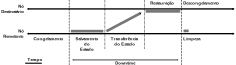
\includegraphics[width=0.8\linewidth]{content/images/cold-migration-flow.pdf}
    \label{fig.coldmigration}
    \fonte{Adaptado de~\citeonline{migrationimages}}
\end{figure}

\subsubsection{\Hotmigration}\label{sec.hotmigration}
Em contraste com a \coldmigration, na \hotmigration, também conhecida como \livemigration, o sistema a ser migrado não precisa ser desligado antes do processo começar. O principal objetivo desse processo é maximizar a performance do sistema durante a migração, melhorar o uso da rede e reduzir o \downtime do sistema~\cite{imran2022live}.

Neste modelo, a migração poder ser classificada de acordo com a técnica utilizada para a transferência dos dados \ie \precopymigration, \postcopymigration e migração híbrida.

\subsubsubsection{\Precopymigration}\label{sec.precopymigration}
Neste modelo, ao receber a requisição de migração, o sistema cria uma pré-imagem do seu estado atual e a envia ao destinatário enquanto continua executando normalmente. Nesta estrutura está contida o esquema de paginação atual do sistema e, por vezes, alguns dados de execução. Conforme o esquema de paginação é modificado no remetente, essa estrutura é atualizada e enviada ao destinatário. Depois disso, é salvo o estado atual completo do sistema, que, então, é enviado ao destino. O sistema é restaurado no destino e o estado do sistema apagado no remetente. 

Esse fluxo de migração faz com que o tempo total de migração seja maior que o do \coldmigration, já que há a retransmissão de dados, em especial páginas de memória. Em contrapartida, o \downtime é reduzido, pois o sistema executa normalmente na parte inicial da migração, quando é feita e enviada a pré-imagem ao destinatário~\cite{singh2022predictive, imran2022live}. A \autoref{fig.precopy} ilustra o fluxo de execução da \precopymigration.

\begin{figure}[bt]
    \centering
    \caption{Fluxo de execução da \precopymigration.}
    \includegraphics[width=0.8\linewidth]{content/images/pre-copy-migration-flow.pdf}
    \label{fig.precopy}
    \fonte{Adaptado de~\citeonline{migrationimages}}
\end{figure}

\subsubsubsection{\Postcopymigration}\label{sec.postcopymigration}
Neste modelo, o remetente cria um estado parcial do sistema em execução e o envia ao destinatário. Nesse estado, está incluso apenas o essencial para a execução inicial do sistema, não abrangendo o esquema de paginação. Quando o sistema é restaurado no destinatário, ocorrerão várias faltas de páginas, as quais resultam em requisições de páginas ao remetente, o qual as envia ao destinatário. Quando todas as páginas são transferidas ao destinatário, o sistema é apagado do remetente~\cite{singh2022predictive, imran2022live}. A \autoref{fig.postcopy} ilustra o fluxo de execução da \postcopymigration.

\begin{figure}[bt]
    \centering
    \caption{Fluxo de execução da \postcopymigration.}
    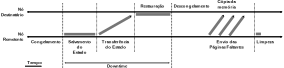
\includegraphics[width=0.8\linewidth]{content/images/post-copy-migration-flow.pdf}
    \label{fig.postcopy}
    \fonte{Adaptado de~\citeonline{migrationimages}}
\end{figure}

\begin{figure}[b]
    \centering
    \caption{Fluxo de execução da migração híbrida.}
    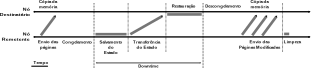
\includegraphics[width=0.8\linewidth]{content/images/hybrid-migration-flow.pdf}
    \label{fig.hybridmigration}
    \fonte{Adaptado de~\citeonline{migrationimages}}
\end{figure}

\subsubsubsection{Migração Híbrida}\label{sec.hybridmigration}
Neste modelo, são utilizadas as técnicas de \precopy e \postcopy em conjunto. Inicialmente, uma pré-imagem do sistema é feita de forma similar ao modelo \precopymigration. Esta pré-imagem é enviada ao destinatário, enqunato o sistema executa normalmente. Em contraste com o método \precopy nesta etapa não são reenviadas as páginas modificadas/atualizadas. Depois, o estado completo do sistema é enviado e as páginas modificadas/atualizadas são requisitadas ao remetente tal como na \postcopymigration. Quando todas as páginas são transferidas ao destinatário, o sistema é apagado do remetente~\cite{singh2022predictive, imran2022live}. A \autoref{fig.hybridmigration} ilustra o fluxo de execução da migração híbrida.




% \mytodo{adicinar seção detalhando o sistema de tasks no background?}